\chapter{Музыкальные композиции}
\label{ch:musical-composition}
Статья посвящена исследованию музыкальных композиций на основе базы знаний международного проекта Викиданные. С помощью SPARQL-запросов, вычисляемых на объектах типа <<музыкальная композиция>> в Викиданных, получен список всех музыкальных композиций, список музыкальных композиций, имеющих композиторов, а также построена пузырьковая диаграмма, показывающая композиторов с наибольшим количеством композиций. Кроме того, решена задача поиска музыкальных лакун в общественном достоянии и выполнена оценка полноты Викиданных.

\section{Экземпляры объекта <<Музыкальные композиции>>}

\marginnote{Используемые в запросах объекты: \wdqName {<<музыкальная композиция>>} {207628};
Используемое свойство: \wdProperty{31}{<<экземпляр>>}}

Построим список всех музыкальных композиций.

\begin{lstlisting}[ language=SPARQL,
                    caption={\href{https://w.wiki/52VP}{Список всех  музыкальных композиций}\protect\footnotemark},
                    label=lst:musical_composition,
                    texcl 
                    ]
# List of all musical compositions
SELECT ?composition ?compositionLabel 
WHERE {
  ?composition wdt:P31 wd:Q207628.
  SERVICE wikibase:label { bd:serviceParam wikibase:language "ru"}
}
\end{lstlisting}%
\footnotetext{Ссылка на SPARQL-запрос: \href{https://w.wiki/52VP}{https://w.wiki/52VP}. \num{5494} записи в 2017 году.}

Наиболее полными и проработанными музыкальными композициями на Викиданных являются: \wdqName{Волшебная флейта}{5064}, \wdqName{К Элизе}{11980}, \wdqName{Реквием}{207875}, \wdqName{Маленькая ночная серенада}{12025}.

Почти пустыми и малоинформативными музыкальными композициями были: \wdqName{Полёт шмеля}{1342275}, \wdqName{Ромео и Джульетта}{763716}, \wdqName{Симфонический эпизод «Завод»}{1845909}, \wdqName{Binks’ Waltz}{28807544}, \wdqName{The Rose-bud March}{28803595}, \wdqName{Leola}{28804177}.

В 2022 году тот же скрипт нашёл \num{453} музыкальные композиции вместо \num{5,5} тысяч в 2017 году. Уменьшение числа композиций связано с тем, что эти объекты Викиданных являются теперь не экземплярами объекта «музыкальные произведения», а его экземплярами различных подклассов «музыкального произведения». При поиске подклассов объекта «музыкальные произведения» можно найти такие жанры: \wdqName{драматико-музыкальное произведение}{58483083}, \wdqName{гимн}{484692}, \wdqName{баллада}{182659}.

Найдём количество музыкальных композиций в каждом жанре с помощью следующего запроса.

\begin{lstlisting}[ language=SPARQL,
                    caption={\href{https://w.wiki/4$PC}{ Количество музыкальных композиций в каждом жанре}\protect\footnotemark},
                    label=lst:music _in_each_subclass,
                    texcl 
                    ]
# Count of pieces of music in each subclass
SELECT ?type (COUNT(?subMusicInstance) AS ?count) ?subMusicLabel 
WHERE {
  ?type wdt:P279* wd:Q207628.	# subclass of musical composition
  ?subMusicInstance wdt:P31 ?type  # instance of that class of
# which this subject is a particular example and member
SERVICE wikibase:label 
{bd:serviceParam wikibase:language "ru, en"}
}
GROUP BY ?type ?subMusicLabel
ORDER BY DESC (?count)
\end{lstlisting}%
\footnotetext{Ссылка на \href{https://w.wiki/4$PC}{SPARQL-запрос}, \num{232} подкласса музыкальных композиций на 2022 год.}

Теперь подсчитаем общее суммарное число музыкальных произведений с учётом музыкальных композиций в подклассах. Для этого добавим в наш скрипт команду \lstinline|SUM()| и удалим лишние строки. Получим такой код:

\begin{lstlisting}[ language=SPARQL,
                    caption={\href{https://w.wiki/4$Q$}{ Суммарное число музыкальных произведений с учётом музыкальных композиций в подклассах}\protect\footnotemark},
                    label=lst:musical_works_for_all_subclasses,
                    texcl 
                    ]
# The total number of musical works for all subclasses 
SELECT (SUM(?count) AS ?sum) WHERE{
  SELECT (COUNT(?music) AS ?count) WHERE {
    ?type wdt:P279* wd:Q207628.  # subclass of musical composition
    ?music wdt:P31 ?type  # instance of that class of which this
# subject is a particular example and member
  }
}
\end{lstlisting}%
\footnotetext{Ссылка на \href{https://w.wiki/4$Q$}{SPARQL-запрос}, \num{135466} музыкальных произведений.}

Можно записать этот код еще короче. Переменная \lstinline|?type| нам не нужна, поэтому можно обойтись без неё, а 4 и 5 строки поменяем местами.

\begin{lstlisting}[ language=SPARQL,
                    caption={\href{https://w.wiki/4$R3}{ Суммарное число музыкальных произведений с учётом музыкальных композиций в подклассах}\protect\footnotemark},
                    label=lst:musical_works_for_all_subclasses,
                    texcl 
                    ]
# The total number of musical works for all subclasses 
SELECT (SUM(?count) AS ?sum) WHERE{
  SELECT (COUNT(?music) AS ?count) WHERE {
    ?music wdt:P31   # instance of
        [ wdt:P279* wd:Q207628 ]. # subclass of
# musical composition
  }
}
\end{lstlisting}%
\footnotetext{Ссылка на \href{https://w.wiki/4$R3}{SPARQL-запрос}, на 1 апреля 2022 года запрос выдает \num{135466} музыкальных произведений.}

По сравнению с 2017 годом \num{5494} записи, число записей увеличилось в несколько раз. Это связано с тем, что за 5 лет было добавлено множество новых музыкальных произведений, а также старых, которые не учли ранее.


\subsection{Поиск музыкальных лакун в общественном достоянии}
Задача состоит в том, чтобы найти такие музыкальные произведения, авторы которых умерли более 70 лет назад, и аудиозапись которых отсутствует на Викискладе. Упорядочить такие произведения от самых старых к новым. Существует практическая выгода и польза от такого скрипта, поскольку видно, какие произведения можно и нужно оцифровывать (с пластинок, кассет) и загружать на Викисклад.

\begin{lstlisting}[ language=SPARQL,
                    caption={\href{https://w.wiki/56Mh}{ Отсутсвующие аудиозаписи музыкальных произведений, авторы которых умерли более 70 лет назад }\protect\footnotemark},
                    label=lst:music_gaps_in_public_domain,
                    texcl 
                    ]
#Search music gaps in public domain
SELECT ?composition ?compositionLabel ?publication
WHERE {
  ?composition wdt:P31 wd:Q207628.  # instance of compostion
  ?composition wdt:P86 ?composer.  # composition has a composer
  ?composition wdt:P577 ?publication.  # composition has a
# publication date
  ?composer wdt:P570 ?death.             # composer has a date
# of death
  MINUS {?composition wdt:P51 []}.  # compositions without audio 
  FILTER(?death < "1947-01-01T00:00:00Z"^^xsd:dateTime)  
# composers that passed away more than 70 years ago
  FILTER(?publication < "1947-01-01T00:00:00Z"^^xsd:dateTime)  
# compositions that were published more thatn 70 years ago
  SERVICE wikibase:label {bd:serviceParam wikibase:language "ru".}
}
ORDER BY ASC(?publication)
\end{lstlisting}%
\footnotetext{Ссылка на \href{https://w.wiki/56Mh}{SPARQL-запрос}, 140 записей.}




\subsection{Полнота Викиданных}
Проанализируем полноту Викиданных.

По данным \href{https://ru.wikipedia.org/wiki/Музыкальный_словарь_Гроува}{<<Музыкального словаря Гроува>>} за всю историю человечества существовало \num{20374} композиторов.

По данным категории \href{https://ru.wikipedia.org/wiki/Категория:Композиторы_по_алфавиту}{<<Композиторы по алфавиту>>} Русской Википедии существует \num{7412} композиторов.

По данным категории \href{https://en.wikipedia.org/wiki/List_of_composers_by_name}{<<List of composers by name>>} Английской Википедии существует \num{4685} композиторов.

Количество музыкальных композиций с заполненным свойством \wdProperty{86}{<<композитор>>} равно \num{3862} \footnote{ Ссылка на \href{https://w.wiki/56Rc}{SPARQL-запрос}.}, и это с учётом того, что один композитор мог написать несколько музыкальных произведений. Например, \href{https://ru.wikipedia.org/wiki/Моцарт,_Вольфганг_Амадей}{Вольфганг Амадей Моцарт} написал \num{95} произведений, что существенно снижает количество уникальных композиторов. Полученное число \num{3862} меньше, чем количество композиторов из русской и английской Википедии, и существенно меньше, чем количество композиторов из \href{https://ru.wikipedia.org/wiki/Музыкальный_словарь_Гроува}{<<Музыкального словаря Гроува>>}, что говорит нам о неполноте Викиданных.

\href{https://w.wiki/56Rj}{SPARQL-запрос} по композициям с заполненным свойством \wdProperty{86}{<<композитор>>} и свойством \wdProperty{495}{<<страна происхождения>>}, имеющим значения \wdqName{<<Российская империя>>}{34266}, \wdqName{<<СССР>>}{15180} или \wdqName{<<Россия>>}{159}, выдал всего лишь \num{8} произведений, что говорит о невозможности анализа русских музыкальных произведений в связи с недостатком данных.

Построим пузырьковую диаграмму композиторов музыкальных композиций.

\begin{lstlisting}[ language=SPARQL, numbers=none,
                    caption={\href{https://w.wiki/56Ry}{ Пузырьковая диаграммп композиторов музыкальных композиций }\protect\footnotemark},
                    label=lst:BubbleChart,
                    texcl 
                    ]
#composers of musical compositions
#defaultView:BubbleChart
SELECT ?composer ?form (COUNT(*) AS ?count) 
WHERE {
  ?composition wdt:P31 wd:Q207628. # instance of composition
  ?composition wdt:P86 ?composer.  # composition has a composer
  OPTIONAL {
  ?composer rdfs:label ?form.  
  FILTER((LANG(?form)) = "ru")
  }
}
GROUP BY ?composer ?form
ORDER BY DESC(?count) ?form
\end{lstlisting}%
\footnotetext{Получено \num{773} записи. Ссылка на SPARQL-запрос: \href{https://w.wiki/56Ry}{https://w.wiki/56Ry}}

Результат работы запроса~\ref{lst:BubbleChart} представлен на рис.~\ref{fig:ComposerOfMusicalCompositions}.

\begin{fullwidth}
\begin{figure*}[ht]
	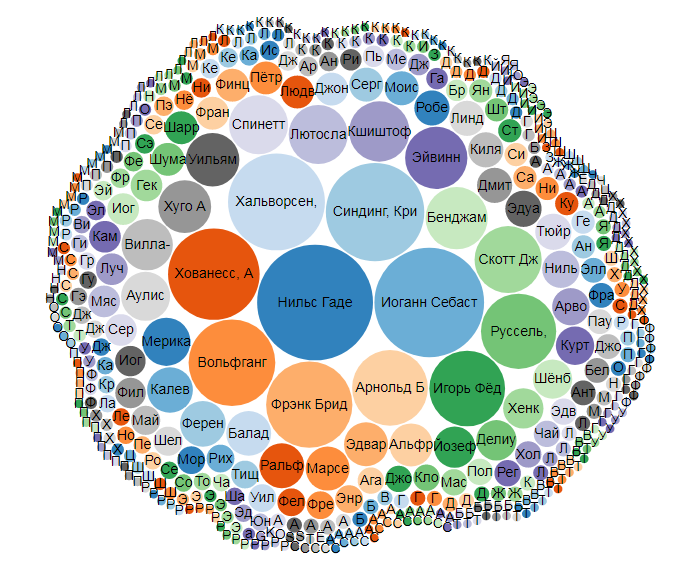
\includegraphics[width=\textwidth]{./chapter/musical_composition/Composer_of_musical_compositions_bubble_diagram.png}
	\caption[Пузырьковая диаграмма композиторов по количеству написанных композиций.]{Размер круга означает количество написанных музыкальных композиций. Диаграмма показывает, что у одних композиторов значительно больше композиций чем у других. В первую пятерку входят \href{https://ru.wikipedia.org/wiki/Гаде,_Нильс}{Нильс Гаде} (\num{173} композиции), \href{https://ru.wikipedia.org/wiki/Бах,_Иоганн_Себастьян}{Иоганн Себастьян Бах} (\num{155} композиций), \href{https://ru.wikipedia.org/wiki/Синдинг,_Кристиан_Август}{Кристиан Август Синдинг} (\num{125} композиций), \href{https://ru.wikipedia.org/wiki/Хальворсен,_Юхан}{Юхан Хальворсен} (\num{121} композиция), \href{https://ru.wikipedia.org/wiki/Хованесс,_Алан}{Алан Хованесс} (\num{108} композиций). Карта построена с помощью запроса~\protect\ref{lst:BubbleChart}.}%
      \label{fig:ComposerOfMusicalCompositions}%
\end{figure*} 
\end{fullwidth}



\subsection{Заполнение Викиданных}
Для того чтобы получить больше записей при выполнении скрипта для поиска музыкальных лакун в общественном достоянии, было решено заполнить свойство \wdProperty{86}{<<композитор>>} у объектов типа \wdqName{<<музыкальная композиция>>}{207628}.

Построим список всех музыкальных композиций с заполненным свойством \wdProperty{86}{<<композитор>>}.

\begin{lstlisting}[ language=SPARQL,
                    caption={\href{https://w.wiki/52VP}{Списки композиций, у которых композитор из России}\protect\footnotemark},
                    label=lst:Compositions_that_has_a_composer_in_Russian,
                    texcl 
                    ]
#Lists of compositions that has a composer in Russian 
SELECT ?composition ?compositionLabel ?composer ?composerLabel 
WHERE {
  ?composition wdt:P31 wd:Q207628. # instance of composition
  ?composition wdt:P86 ?composer.  # composition has a composer
  SERVICE wikibase:label {bd:serviceParam wikibase:language "ru".}
}
}
\end{lstlisting}%
\footnotetext{\href{https://w.wiki/56Sb}{SPARQL-запрос} на 30 октября 2017 года выдает \num{3965} записей.}



\subsection{Будущая работа}
\begin{enumerate}
\item Найти список музыкальных композиций, созданных во время эпохи классицизма (XVII—XVIII века).
Свойство: \wdProperty{571}{<<дата создания>>}.
\item Найти композитора, который написал больше симфоний чем остальные.
Свойства: \wdProperty{31}{<<экземпляр>>}, \wdProperty{86}{<<композитор>>}.
\item Построить гистограмму, на которой отображается количество музыкальных композиций группы The Beatles по году публикации.
Свойства: \wdProperty{175}{<<исполнитель>>}, \wdProperty{577}{<<дата публикации>>}.
\end{enumerate}
